\documentclass[11pt, oneside]{article} 
\usepackage{geometry}
\geometry{letterpaper} 
\usepackage{graphicx}
	
\usepackage{amssymb}
\usepackage{amsmath}
\usepackage{parskip}
\usepackage{color}
\usepackage{hyperref}

\graphicspath{{/Users/telliott/Github/precalculus/fig/}}
% \begin{center} \includegraphics [scale=0.4] {gauss3.png} \end{center}

\title{Special points}
\date{}

\begin{document}
\maketitle
\Large
Special points in triangles include the:

$\circ$ \  orthocenter:  where altitudes cross

$\circ$ \  centroid:  where the medians (lines to the midpoints of sides) cross
\begin{center} 
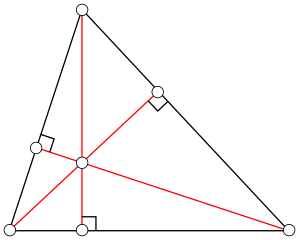
\includegraphics [scale=0.5] {orthocenter.png}
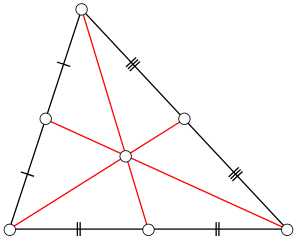
\includegraphics [scale=0.5] {centroid.png} 
\end{center}

$\circ$ \  circumcenter:  the circle where all three vertices lie, also, where perpendiculars to side midpoints cross

$\circ$ \  incenter:  where angle bisectors cross
\begin{center} 
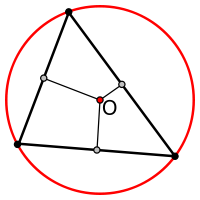
\includegraphics [scale=0.5] {circumcenter.png}
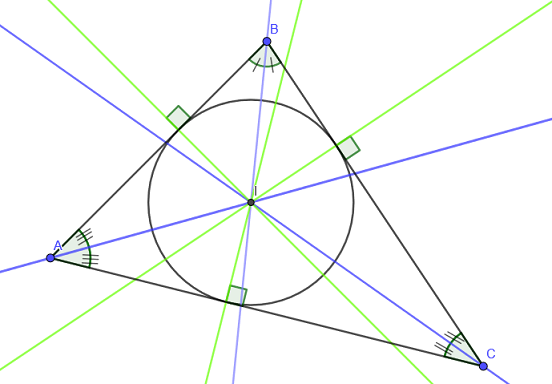
\includegraphics [scale=0.5] {incenter.png} \end{center}

Euler showed that the first three of these points lie on one line.
\begin{center} 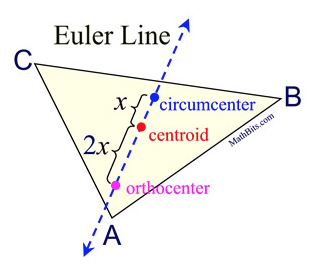
\includegraphics [scale=0.6] {euler_line.png} \end{center}

\subsection*{centroid}
We'll start with the centroid.  The centroid is where bisectors of opposing sides cross.

Consider the triangle in the figure below (left panel).  

\begin{center} 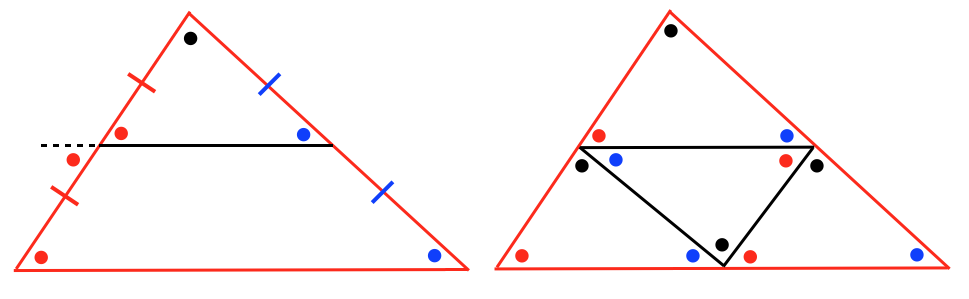
\includegraphics [scale=0.4] {midpoints1.png} \end{center}

Draw a line segment parallel to the base and connecting to the midpoint of the left side.  Then, by the alternate interior angle theorem and the vertical angle theorem, the two angles marked with red dots in the middle are equal to the red dotted angle at the base.

Therefore, by three angles the same, the small upper triangle is similar to the large one.  The ratio of similar sides is $1:2$.

But this can be done on the right side as well, and then the same for all three vertices of the original triangle (right panel).  

By the triangle sum theorem and also by the alternate interior angle theorem, the angles in the interior triangle are equal to other angles as indicated.  By shared sides, the four small triangles are congruent.

Now draw lines from each vertex to the midpoint of the opposing side.  $GHIA$ is a parallelogram, by the angle equalities just proven.  The two diagonals of a parallelogram cross at their midpoints.  Therefore $O$ is the midpoint of the side $GI$ and the same line that connects $A$ to midpoint $H$ also connects $H$ to midpoint $O$.

\begin{center} 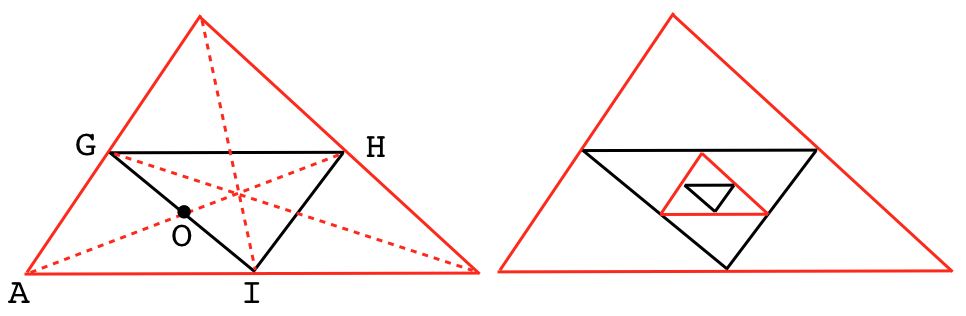
\includegraphics [scale=0.4] {midpoints2.png} \end{center}

Therefore the centroid of $\triangle GHI$ is also the centroid of the parent.  This process can be repeated as many times as we please (right panel).  The triangles get smaller and eventually tend to a point.  That point is on all three midpoint segments.  Therefore, the centroid is a single point.

\subsection*{algebra of the centroid}

We can locate the centroid by imagining that we find successive midpoints of a length from opposite ends left and right.  The first point is at $1/2$ of the length (from the left), the second comes back from $1$ by $1/4$ so is at $0.75$ (at the right), the third is at $0.5 + 1/8$ (from the left), so every second round we get closer to the centroid  by advancing from the left by
\[ S = \frac{1}{2} +  \frac{1}{8} +  \frac{1}{32}  + \dots \]

Now, we can either assume this sum is finite (for now) or recognize that it is certainly smaller than 
\[ \frac{1}{2} +  \frac{1}{4} +  \frac{1}{8}  + \dots = 1 \]

\begin{center}
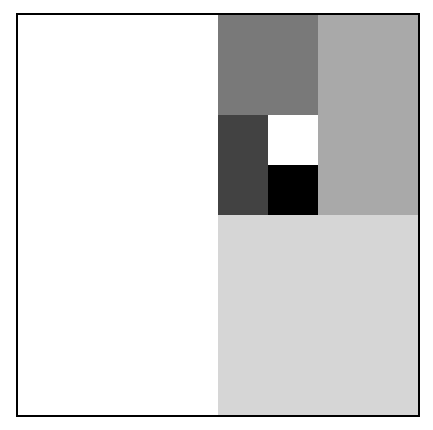
\includegraphics [scale=0.4] {series1.png}
\end{center}

So if
\[ S = \frac{1}{2} +  \frac{1}{8} +  \frac{1}{32}  + \dots \]
then
\[ 2S = 1 +  \frac{1}{4} +  \frac{1}{16}  + \dots \]
and
\[ 3S = 1S + 2S = 1 +  \frac{1}{2} +  \frac{1}{4} +  \frac{1}{8} + \frac{1}{16}   + \dots \]
That is, $3S = 1 + 1$, so $S = 2/3$.


$\square$

\subsection*{orthocenter}
An altitude of a triangle is a line extended from a vertex so as to form a right angle with the opposing side.  The \emph{orthocenter} is the point where the three altitudes of a triangle meet.

Assume for now that the three altitudes \emph{do} meet at a single point, we will come back to this question later.
\begin{center} 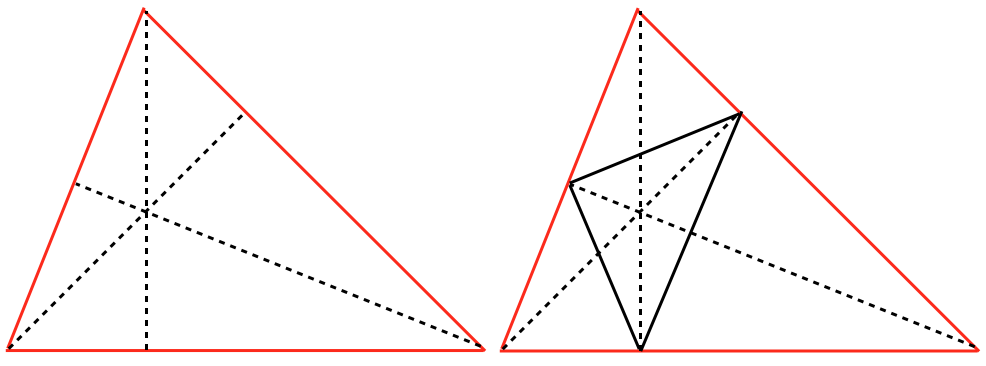
\includegraphics [scale=0.4] {altitude_proof_1.png} \end{center}

Above we have drawn the altitudes (left panel) and connected the points where the altitudes meet the sides.  We can prove something interesting about the inset triangle.  We will prove that the incenter of that triangle is equal to the orthocenter of the bigger one.

\begin{center} 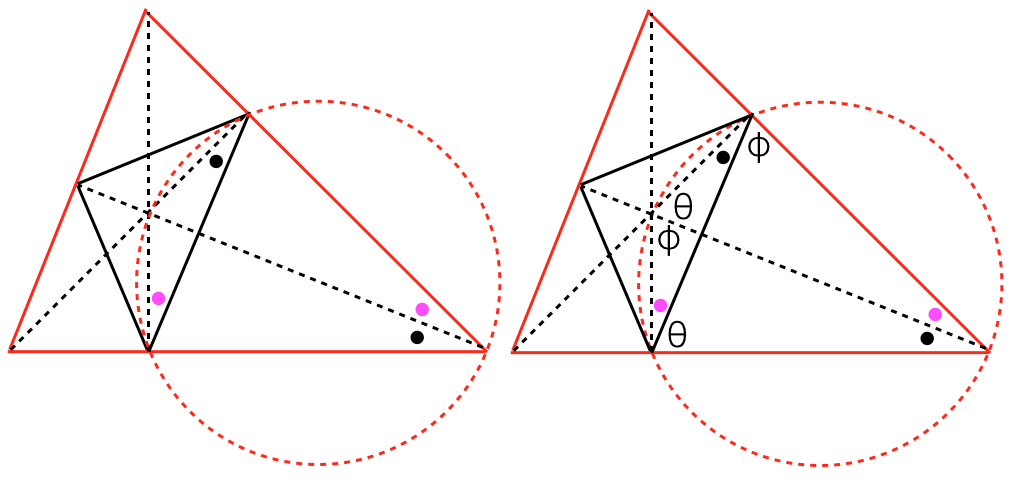
\includegraphics [scale=0.4] {altitude_proof_2.png} \end{center}

The dotted lines form right angles at the sides.  Therefore, we can use the common dotted line as a diameter and draw a circle that includes all four points.

Despite what it looks like, the figure is not symmetrical across the diameter.  For example, the angles marked with black dots and those marked with magenta dots are not equal.

However, now we can use our theorems about arcs subtended by an angle on the perimeter of the circle.  The two angles marked with black dots subtend the same arc.  Similarly for magenta.  The same is also true for the pairs of angles marked $\phi$ and $\theta$.

We use symmetry to fill in some more equalities.

\begin{center} 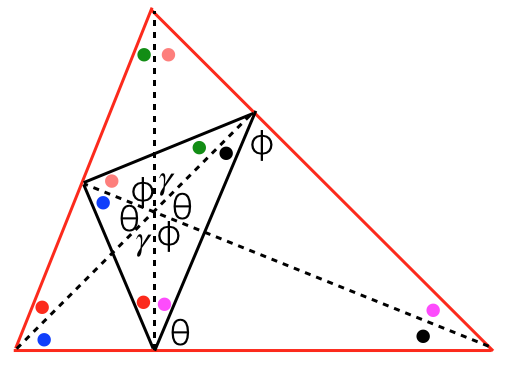
\includegraphics [scale=0.4] {altitude_proof_3.png} \end{center}

This looks like a mess.  But let us look more carefully at one set of angles, $\phi$ and the black and green.

\begin{center} 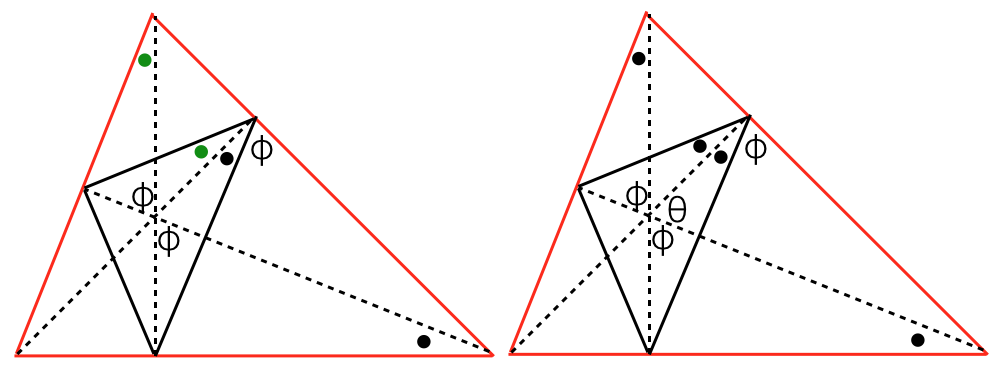
\includegraphics [scale=0.4] {altitude_proof_4.png} \end{center}

Notice that, at the bottom, $\phi$ is complementary to black, but the top left, $\phi$ is complementary to green.  Hence black and green must be equal (right panel).  We carry out the same exercise for $\theta$, red and pink.

\begin{center} 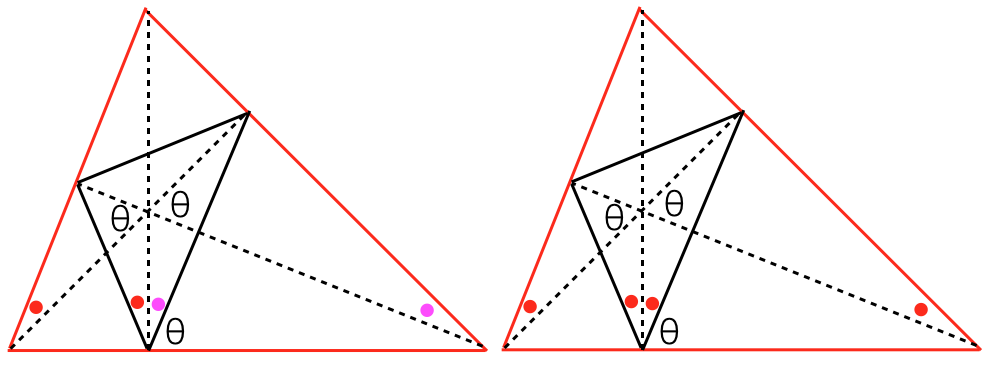
\includegraphics [scale=0.4] {altitude_proof_5.png} \end{center}

And then, for $\gamma$, blue and salmon.
\begin{center} 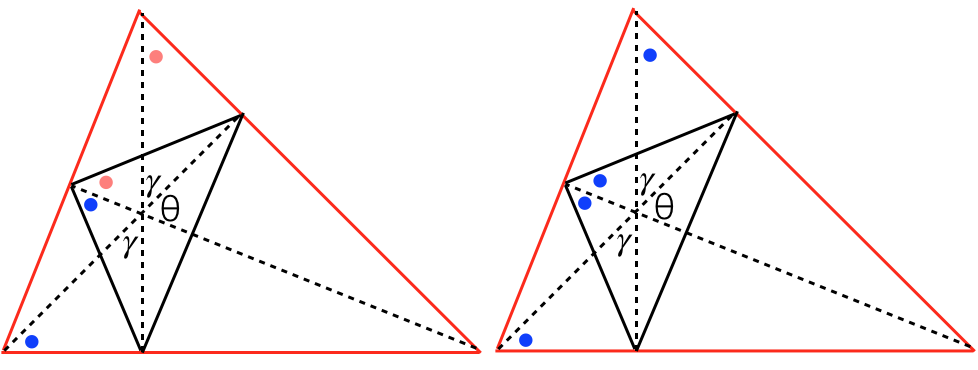
\includegraphics [scale=0.4] {altitude_proof_6.png} \end{center}

Restoring dots
\begin{center} 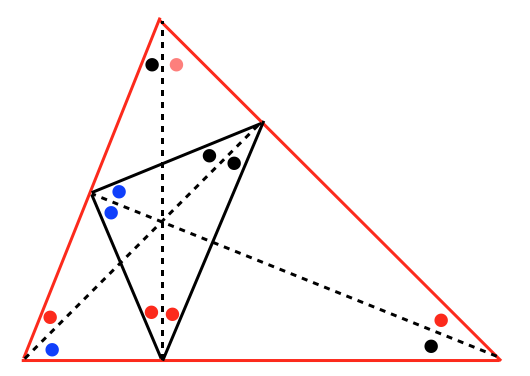
\includegraphics [scale=0.4] {altitude_proof_7.png} \end{center}

We can see that the dotted lines are angle bisectors for the small triangle.

$\square$

\subsection*{Euler's proof}

Below we give an alternative proof, due to Euler, which is stunning, following

\url{https://artofproblemsolving.com/wiki/index.php/Orthocenter}

Borrowing their figure:

\begin{center} 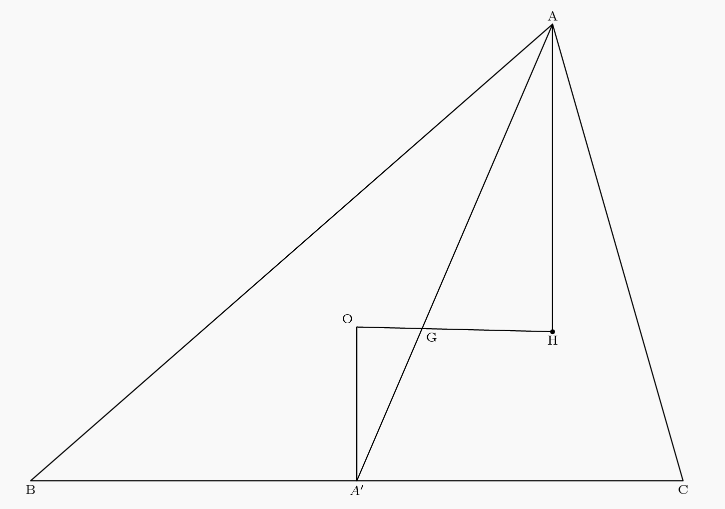
\includegraphics [scale=0.35] {circumcenter2.png} \end{center}
The orientation is reversed from what we had above.  First, the point $O$ is the circumcenter of the triangle:  the center of the circle which contains all three vertices of the triangle.  

Clearly, this circle  has a center.  The classic construction is to bisect each side (here $BC$ is bisected at $A'$), and erect a perpendicular.  The point where the three perpendiculars cross is the circumcenter, which is the center of the circle.  

\begin{center} 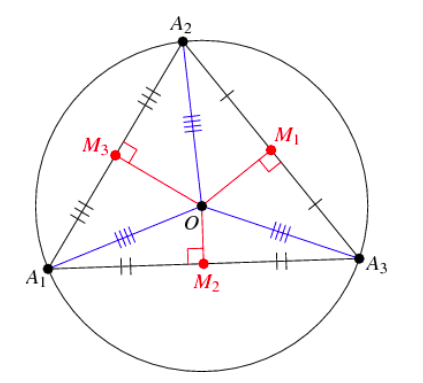
\includegraphics [scale=0.45] {three_point_circle2.png} \end{center}

So, assume we have done this and that point is $O$.

The next point, $G$, is the centroid.  One way to find this point is to draw all three lines connecting vertices with the midpoints of the opposite side ($AA'$).  However, if you recall, the distance from the vertex $A$ to $G$ is twice the distance from the midpoint $A'$ to $G$.  Hence we draw point $G$ using arithmetic.

Now, extend $OG$ by twice its length, to $H$.  ($2OG = GH$).
\begin{center} 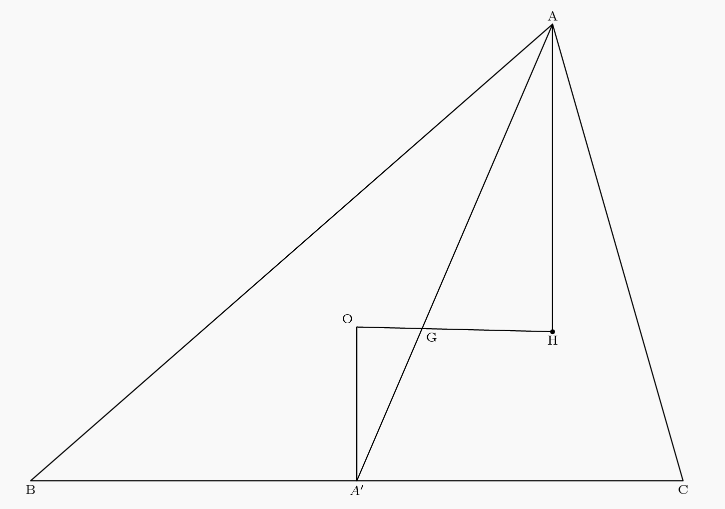
\includegraphics [scale=0.35] {circumcenter2.png} \end{center}
Because $AG$ is twice $A'G$ and $GH$ is twice $OG$ and the two triangles share both angle $\angle OGA'$ (equal to $\angle AGH$), they are similar triangles.  

Since $\angle A'OG$ is a right angle, therefore so is $\angle AHG$.  This means that $AH$ is perpendicular to $BC$.  Thus, $AH$ is a part of the altitude from $A$ to $BC$ (the whole altitude is not shown).

The same construction could be done for the other two vertices, each time ending at $H$.  This shows that $H$ is unique, and that $H$ is on all three altitudes.

This proof also demonstrates that the orthocenter, centroid and circumcenter lie on a single line, and that the distance from centroid to orthocenter is twice that from centroid to circumcenter.


\end{document}